%!TEX encoding = IsoLatin

%% Document is article 
\documentclass[a4paper]{article}

%% ----------------------------------------------------- PACKAGES ----------------------------------------------------- %%
\usepackage{coolArticle}
\usepackage[ruled]{algorithm2e}
\usepackage{verbatim}


%% ---------------------------------------------------- DOCUMENT ---------------------------------------------------- %%
\begin{document}

	\noindent \textsc{Gallois-Montbrun} Gr�goire\\
	\textsc{Faury} Louis 
		\titlebox{0.6}{Model Predictive Control}{Exercise \#4 - \textcolor{blue}{Group 2}}
	
	\section{Ex.1 : Implement MPC}
	{
		\paragraph{} We consider the following discrete-time linear time-invariant system : 
		\begin{equation}
			x^+ = \begin{bmatrix} 0.9752 & 1.4544 \\ -0.0327 & 0.9315 \end{bmatrix} + \begin{bmatrix} 0.0248 \\ 0.0327\end{bmatrix}u
		\end{equation}
		with constraints : 
		\begin{equation}
			\begin{aligned}
				\mathbb{X} &= \{x\, \vert \, \vert x_1 \vert \leq 5, \, \vert x_2 \vert \leq 0.2 \}\\
				\mathbb{U} &= \{ u\, \vert \, \vert u \vert \leq 1.75\}
			\end{aligned}
		\end{equation}
		
		\paragraph{} We are going to implement a MPC controller for this system with horizon $N=10$ and cost function : 
		\begin{equation}
			I(x,u) = 10 x^Tx + u^T u
		\end{equation}
		
		\paragraph{} Let us first compute the terminal controller, terminal weight function and the terminal set that ensure recursive feasibility and stability of the closed loop system. Thanks to the last exercise session, their derivation is straight-forward : the terminal controller $K_{lqr}$ and the terminal weight function $V_{lqr}(x) = x^TPx$ are obtained thanks to the \texttt{dlqr($\cdot$)} Matlab function. The terminal set is therefore obtained by computing the maximum invariant set for the system : 
		\begin{equation}
			x^+ = (A+BK_{lqr})x
		\end{equation}
		
Figure (\ref{fig::sets}) displays both feasible and computed terminal sets.
		
		\begin{figure}[h!]
		\centering
			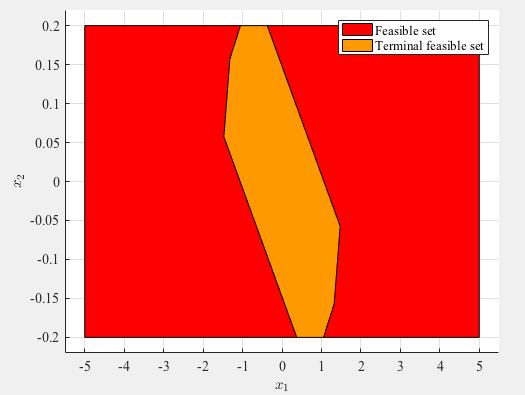
\includegraphics[scale=0.4]{sets}
			\caption{Feasible set and terminal set}
			\label{fig::sets}
		\end{figure}
		
		\paragraph{} The MPT library allows us to check that our computations are correct : 
		{\small 
		\begin{verbatim}
			Boolean value for equality between sets (=1 if sets are equal) :
   			1

			MPT terminal state :
   			37.0252   68.3850
  			 68.3850  407.1177

			Our terminal state :
 			  37.0252   68.3850
  			 68.3850  407.1177

			MPT terminal gain :
  			 -1.6478  -11.8344

			Our terminal gain :
  			 -1.6478  -11.8344
		\end{verbatim}
		}
		
		
		\paragraph{} We now proceed on implementing the MPC algorithm. We use Matlab optimization function \texttt{quadprog} which solves the optimization program : 
		\boxedeq{red}
		{
			\begin{aligned}
				fval = &\min_z& \frac{1}{2}z^THz + h^Tz \\
					  & \text{s.t } &Gz \leq g \\
					  &		     &Tz = t
			\end{aligned}
		}
		
                \begin{figure}[h!]
			\begin{minipage}{0.45\linewidth}
			{\centering
				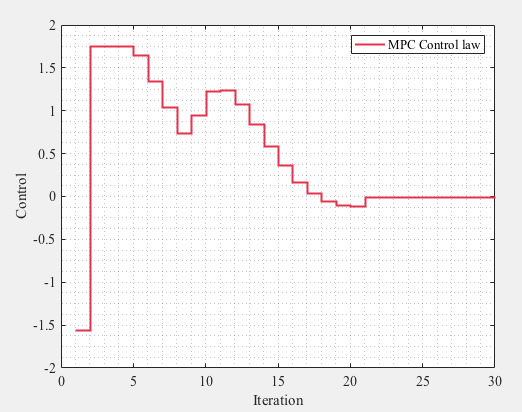
\includegraphics[width=1\linewidth]{MPC_control}
				\caption{Control sequence retrieved from the closed loop MPC controller}
				\label{fig::MPC_control}
			}
			\end{minipage}\hfill
			\begin{minipage}{0.45\linewidth}
			{	\centering
				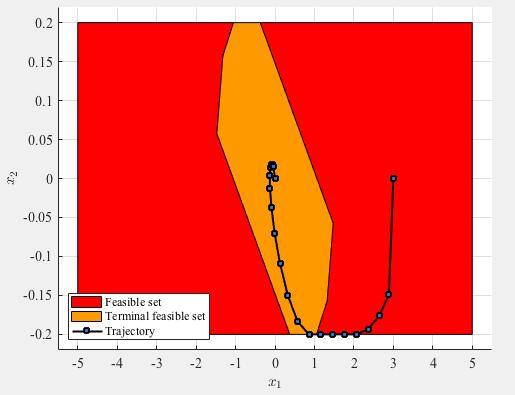
\includegraphics[width=1\linewidth]{MPC_trajectory}
				\caption{Position and velocity of the controlled system}
				\label{fig::MPC_trajectory}
			}
			\end{minipage}
		\end{figure}
		
		We therefore need to express our initial optimization program 
		\begin{equation}
			\begin{aligned}
				&\min_{u, x} \sum_{i=0}^{N-1} \left\{  x_i^TQx_i + u_i^T Ru_i \right\}+x_N^TPx_N \\
				& \text{ s.t }  \left\{
					\begin{aligned}
						&\forall i \in\{0,\hdots, N\}, \, x_{i+1} = Ax_i + Bu_i \\
						&\forall i \in\{1,\hdots, N\}, \,  (x_i,u_{i-1}) \in \mathbb{X} \times\mathbb{U} \\
						&x_N \in \mathcal{X}_f
					\end{aligned}\right.
			\end{aligned}
		\end{equation}
		as such, with $Q = 10\cdot I_2$, $R=1$. This leads to the following expressions : 
		\begin{equation}
		\left\lVert
			\begin{aligned}
				z &= \begin{pmatrix} x_{11}, x_{12}, \hdots x_{N2}, u_0, \hdots u_{N-1}\end{pmatrix}^T \in \mathbb{R}^{3N}\\[10pt]
				H &= 2\begin{pmatrix}
					Q &  0 & 0 & 0& 0 & 0 & 0\\
					0 & \ddots & \ddots  & \ddots & \ddots &\ddots& \vdots \\
					0 & \ddots & \ddots  & \ddots   \ddots & \ddots &\ddots& \vdots \\
					0 & \ddots & \ddots  & Q & \ddots & \ddots & \vdots\\
					0 & \ddots & \ddots & \ddots & R & \ddots& \vdots \\
					0 & \ddots & \ddots & \ddots & \ddots & \ddots & 0 \\
					0 & \hdots & \hdots & \hdots & \hdots & 0 & R
				\end{pmatrix} \in\mathcal{M}_{3N,3N}(\mathbb{R}) \\[10pt]
				h &= 0_{\mathbb{R}^{3N}} \\[10pt]
				T &= \begin{pmatrix}
						I_2  & 0 & \hdots & 0 & -B & 0 & \hdots & 0 \\
						-A & \ddots  & \ddots & \ddots & \ddots & \ddots & \ddots & \vdots \\
						0 & \ddots & \ddots  & \ddots & \ddots & \ddots & \ddots & \vdots \\
						0 & \hdots & -A & I_2  & 0 & \hdots & \hdots & -B
					\end{pmatrix} \in\mathcal{M}_{2N,3N}(\mathbb{R}) \\[10pt]
				t &= \begin{pmatrix} Ax_0 & 0 & \hdots & 0 \end{pmatrix}^T \in\mathbb{R}^{2N} \\[10pt] \\
				G &= \begin{pmatrix}
					C &  0 & 0 & 0& 0 & 0 & 0\\
					0 & \ddots & \ddots  & \ddots   \ddots & \ddots &\ddots& \vdots \\
					0 & \ddots & C  & \ddots & \ddots & \ddots & \vdots\\
					0 & \ddots & \ddots  & F & \ddots & \ddots & \vdots\\
					0 & \ddots & \ddots & \ddots & D & \ddots& \vdots \\
					0 & \ddots & \ddots & \ddots & \ddots & \ddots & 0 \\
					0 & \hdots & \hdots & \hdots & \hdots & 0 & D
				\end{pmatrix}\\[10pt]
				g &= \begin{pmatrix} c & \hdots & c & f & d & \hdots & d \end{pmatrix}^T
			\end{aligned}\right.
		\end{equation}
		where we took the following notations : 
		\begin{equation}
			\begin{aligned}
				&\mathbb{X} = \{ x \, \vert \, Cx \leq c \} \\
				&\mathbb{U} = \{ u \, \vert \, Du \leq d\}\\
				&\mathcal{X}_f = \{ x \, \vert \, Fx \leq f \}
			\end{aligned}
		\end{equation}
	
	
Figures (\ref{fig::MPC_control})  and (\ref{fig::MPC_trajectory}) show the control sequence applied to the system controlled by the closed loop MPC controller and  the resulting trajectory. Initial state is $(3,0)$ and trajectory and control are considered for the 30 first time steps. We notice that all contraints on state  and control are always satisfied. The state converges to position $(0,0)$.

		
	}
	
		\section{Ex.2 : Implement MPC using YALMIP}
	{
		\paragraph{}
		The exact same controller as in previous exercise was implemented using \textbf{YALMIP toolbox.}  	The syntax used for implementing the problem was directly inspired of the examples available online. \textbf{The same results were obtained using this library thus confirming our implementation of exercise 1}. Retrieved trajectory and control are displayed on Figures (\ref{fig::YALMIP_control}) and (\ref{fig::YALMIP_trajectory}).
	}
	
	                \begin{figure}[h!]
			\begin{minipage}{0.45\linewidth}
			{\centering
				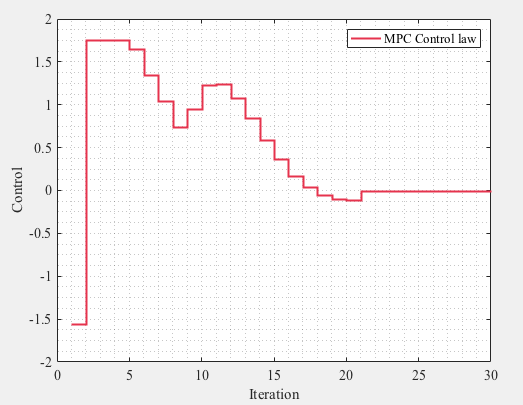
\includegraphics[width=1\linewidth]{YALMIP_control}
				\caption{Control sequence retrieved from the closed loop MPC controller}
				\label{fig::YALMIP_control}
			}
			\end{minipage}\hfill
			\begin{minipage}{0.45\linewidth}
			{	\centering
				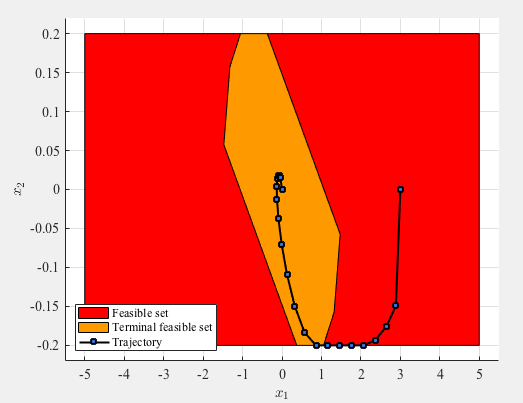
\includegraphics[width=1\linewidth]{YALMIP_trajectory}
				\caption{Position and velocity of the controlled system}
				\label{fig::YALMIP_trajectory}
			}
			\end{minipage}
		\end{figure}



\end{document}